\documentclass{article}
\usepackage{graphicx}
\usepackage[a4paper, left=2cm, right=2cm, top=2cm, bottom=2cm]{geometry}

\usepackage[utf8]{inputenc}
\usepackage[greek,english]{babel}
\usepackage{alphabeta}
\usepackage{amsmath}
\usepackage{caption}
\usepackage{subcaption}
\usepackage{xcolor}
\usepackage{mathabx}
\usepackage{amssymb}
\usepackage{enumitem}

\captionsetup{labelformat=empty}
\subcaptionsetup{labelformat=empty}

\title{\textbf{Προσαρμοστικός Έλεγχος - Εργασία 1: Θεωρία Ευστάθειας}}
\author{\textbf{Ονοματεπώνυμο}: Βραχωρίτη Αλεξάνδρα (A.M.: 1092793)}
\date{16 Νοεμβρίου 2025}

\begin{document}
\maketitle
\section{Άσκηση 1η}
Δίνεται το σύστημα:

\begin{equation*}
\dot{x_1} = x_2 + c x_1 (x_1^2 + x_2^2) 
\end{equation*}

\begin{equation*}
\dot{x_2} = - x_1 + c x_2 (x_1^2 + x_2^2)   
\end{equation*}

\subsection{Να βρεθούν τα σημεία ισορροπίας (equilibrium points) του συστήματος.}
Σημείο ισορροπίας (equilibrium point) \(x_e\) είναι μια κατάσταση στην οποία, αν το σύστημα βρεθεί τη στιγμή \(t_e\), θα παραμείνει εκεί \(\forall\,t \geq t_e\), εφόσον δεν υπάρξουν μεταβολές στο σύστημα ή στις εισόδους του. Αυτό μαθηματικά μπορούμε να το εκφράσουμε λέγοντας ότι η παράγωγος ως προς τον χρόνο (για κάθε μεταβλητή του συστήματος) θα πρέπει να παραμένει σταθερή. Για την εύρεση, λοιπόν, του σημείου ισορροπίας του παραπάνω συστήματος θα πρέπει:

\hfill\break
\begin{math}
    \begin{cases}
        \dot{x}_1 = 0 \\
        \dot{x}_2 = 0
    \end{cases} \Rightarrow
    \begin{cases}
        x_2 + c x_1 (x_1^2 + x_2^2) = 0 \\
        - x_1 + c x_2 (x_1^2 + x_2^2) = 0
    \end{cases} \Rightarrow
    \begin{cases}
        x_2 = 0\,\,\,\text{και}\,\,\,c x_1 (x_1^2 + x_2^2) = 0 \\
        - x_1 = 0\,\,\,\text{και}\,\,\,c x_2 (x_1^2 + x_2^2) = 0
    \end{cases} \Rightarrow \\[10pt]
    \begin{cases}
        x_2 = 0\,\,\,\text{και}\,\,\,c x_1^3 = 0 \\
        x_1 = 0\,\,\,\text{και}\,\,\,c x_2^3 = 0
    \end{cases} \Rightarrow
    \begin{cases}
        x_2 = 0\,\,\,\text{και}\,\,\,x_1 = 0 \\
        x_1 = 0\,\,\,\text{και}\,\,\,x_2 = 0
    \end{cases}
\end{math}

\hfill\break
Άρα, μοναδικό σημείο ισορροπίας του συστήματος είναι το \((x_1, x_2) = (0, 0)\).

\subsection{Να μελετηθεί η ευστάθεια του συστήματος για τα διάφορα c.}
Αρχικά, θα πρέπει να μελετήσουμε την υποψήφια συνάρτηση Lyapunov για να δούμε αν πραγματικά μπορούμε να την αξιοποιήσουμε για την μελέτη της ευστάθειας του συστήματος. Τα κριτήρια που πρέπει να ικανοποιεί είναι:

\begin{itemize}
    \item να είναι θετικά ορισμένη (\(V(x) > 0\))

    \hfill\break    
    \(\forall (x_1, x_2) \neq (0, 0) \): \(V(x) = \frac{x_1^2+x_2^2}{2} > 0\)
    \item να έχει συνεχείς μερικές παραγώγους
    
    \hfill\break
    \begin{math}
        \frac{\partial V(x)}{\partial x_1} = \frac{1}{2}(2x_1) = x_1 \\[10pt]
        \frac{\partial V(x)}{\partial x_2} = \frac{1}{2}(2x_2) = x_2
    \end{math}, όπου είναι πράγματι συνεχείς, αφού \(x_1, x_2 \in \Re\)
\end{itemize}

\hfill\break
Έμεινε κάτι ακόμη, η παράγωγος της υποψήφιας συνάρτησης, που όμως εξαρτάται από την σταθερά c. Συγκεκριμένα

\hfill\break
\begin{math}
    \dot{V}(x) = \nabla V(x) f(x) = x_1 \dot{x_1} + x_2 \dot{x_2} = x_1 (x_2 + c x_1 (x_1^2 + x_2^2)) + x_2 (- x_1 + c x_2 (x_1^2 + x_2^2)) = c (x_1^2 + x_2^2)^2
\end{math}

\subsubsection{\textbf{\(c = 0\)}}
Στην περίπτωση αυτή η V(x) είναι αρνητικά ημιορισμένη (\(V(x) = 0,\,\,\,\forall\,x \neq 0\)), άρα το σύστημα είναι \textbf{ευσταθές}.

\subsubsection{\textbf{\(c > 0\)}}
Στην περίπτωση αυτή η V(x) είναι θετικά ορισμένη (\(V(x) > 0,\,\,\,\forall\,x \neq 0\)), άρα το σύστημα είναι \textbf{ασταθές}.

\subsubsection{\textbf{\(c < 0\)}}
Στην περίπτωση αυτή η V(x) είναι αρνητικά ορισμένη (\(V(x) < 0,\,\,\,\forall\,x \neq 0\)), άρα το σύστημα είναι \textbf{ασυμπτωτικά ευσταθές}.

\section{Άσκηση 2η}
Δίνεται το σύστημα:

\begin{equation*}
    \dot{x_1} = - x_1 = f_1(x_1, x_2)
\end{equation*}

\begin{equation*}
    \dot{x_2} = (x_1 x_2 - 1) x_2^3 + (x_1 x_2 - 1 + x_1^2)x_2 = f_2(x_1, x_2)
\end{equation*}

\subsection{Δείξε ότι το \(x = 0\) είναι μοναδικό σημείο ισορροπίας.}
\hfill\break
\begin{math}
    \begin{cases}
        \dot{x}_1 = 0 \\
        \dot{x}_2 = 0
    \end{cases} \Rightarrow
    \begin{cases}
        - x_1 = 0 \\
        (x_1 x_2 - 1) x_2^3 + (x_1 x_2 - 1 + x_1^2)x_2 = 0
    \end{cases} \Rightarrow
    \begin{cases}
        x_1 = 0 \\
        (x_1 x_2 - 1) x_2^3 = 0\,\,\,\text{και}\,\,\,(x_1 x_2 - 1 + x_1^2)x_2 = 0
    \end{cases} \Rightarrow \\[10pt]
    \begin{cases}
        x_1 = 0 \\
        (0 x_2 - 1) x_2^3 = 0\,\,\,\text{και}\,\,\,(0 x_2 - 1 + 0^2)x_2 = 0
    \end{cases} \Rightarrow
    \begin{cases}
        x_1 = 0 \\
        x_2 = 0
    \end{cases}
\end{math}

\subsection{Δείξε, χρησιμοποιώντας γραμμικοποίηση, ότι το \(x = 0\) είναι ασυμπτωτικά ευσταθές.}
Αρχικά, θα βρούμε τον πίνακα \(\textbf{A}\)

\begin{equation*}
    \textbf{A} =
    \begin{bmatrix}
        \frac{\partial f_1(x)}{\partial x_1} & \frac{\partial f_1(x)}{\partial x_2} \\
        \frac{\partial f_2(x)}{\partial x_1} & \frac{\partial f_2(x)}{\partial x_2}
    \end{bmatrix}
\end{equation*}

\hfill\break
όπου \(f_1(x_1, x_2) = \dot{x_1}\) και \(f_2(x_1, x_2) = \dot{x_2}\), άρα
\begin{math}
    \textbf{A} =
    \begin{bmatrix}
        -1 & 0 \\
        x_2^4 + x_2^2 + 2 x_1 x_2 & 4 x_1 x_2^3 - 3 x_2^2 + 2 x_1 x_2 - 1 + x_1^2
    \end{bmatrix}
\end{math},

\hfill\break
ο οποίος γύρω από το σημείο ισορροπίας είναι
\begin{math}
    \textbf{A} =
    \begin{bmatrix}
        -1 & 0 \\
        0 & -1
    \end{bmatrix}
\end{math}. Το σύστημα \(\dot{\textbf{x}} = \textbf{A}\textbf{x}\) είναι γραμμικό γύρω από το σημείο ισορροπίας και ο πίνακας \(\textbf{A}\) είναι Hurwitz, αφού οι ιδιοτιμές του είναι \(λ_1 = λ_2 = -1 < 0\). Έτσι, συμπεραίνουμε ότι ο σύστημα είναι ασυμπτωτικά ευσταθές.

\subsection{Δείξε ότι το σύνολο \(Γ = \{\textbf{x} \in \Re^2\,\,|\,\,x_1x_2 \geq 2\}\) είναι θετικά αμετάβλητο.}
Έστω \(z = x_1x_2\), άρα

\hfill\break
\begin{math}
    \dot{z} = x_2\dot{x_1} + x_1\dot{x_2} = x_2 (-x_1) + x_1 [(x_1 x_2 - 1) x_2^3 + (x_1 x_2 - 1 + x_1^2)x_2] \Rightarrow \\[10pt]
    \dot{z} = z [x_1^2 + (z-1) x_2^2 + (z-2)]
\end{math}

\hfill\break
και ισχύει \(z \geq 2\), άρα \(z - 1 \geq 1\), \(z - 2 \geq 0\) και \(x_1^2 \geq 0\), \(x_2^2 \geq 0\). Επομένως \(\dot{z} \geq 0,\,\,\forall\,x_1,\,x_2\). Κάποια χρονική στιγμή \(t_0,\,\,z(t_0) = x_1(t_0) x_2(t_0) = z_0 \geq 2\). Άρα, \(\forall\,t \geq t_0,\,\,\dot{z}(t) \geq 0\) και \(0 < 2 \leq z(t)\), δηλαδή η \(z(t)\) είναι μη φθίνουσα συνάρτηση κατά μήκος του συνόλου Γ. Αυτό σημαίνει πως το Γ είναι ένα θετικά αμετάβλητο σύνολο, γιατί προχωρώντας στον χρόνο η τιμή του \(z(t)\) παραμένει μέσα σε αυτό, δηλαδή έχει τιμές μεγαλύτερες του 2.

\subsection{Είναι το \(x = 0\) συνολικά ασυμπτωτικά ευσταθές (globally asymptotically stable);}
Τι σημαίνει ένα σημείο να είναι συνολικά ασυμπτωτικά ευσταθές; Ανεξάρτητα από το σημείο εκκίνησης (starting point) στον χώρο καταστάσεων, η τροχιά του συστήματος θα καταλήγει πάντα στο σημείο ισορροπίας \((x_1, x_2) = (0, 0)\). Όμως, στο προηγούμενο ερώτημα αποδείξαμε πως αν το σημείο εκκίνησης ανήκει στο σύνολο Γ, τότε η τροχιά του συστήματος δεν καταλήγει στο σημείο ισορροπίας. Δεν βρίσκεται καν κοντά σε αυτό. Επομένως, το σημείο ισορροπίας δεν είναι συνολικά ασυμπτωτικά ευσταθές.

\section{Άσκηση 3η}
\subsection{Σύστημα (Α)}
Δίνεται το σύστημα:

\begin{equation*}
    \dot{x_1} = x_1 - x_1^3 + x_2 = f_1(x_1, x_2)
\end{equation*}

\begin{equation*}
    \dot{x_2} = 3x_1 - x_2 = f_2(x_1, x_2)
\end{equation*}

\subsubsection{Να βρεθούν τα σημεία ισορροπίας (equilibrium points) του συστήματος.}
\hfill\break
\begin{math}
    \begin{cases}
        \dot{x}_1 = 0 \\
        \dot{x}_2 = 0
    \end{cases} \Rightarrow
    \begin{cases}
        x_1 - x_1^3 + x_2 = 0 \\
        3x_1 - x_2 = 0
    \end{cases} \Rightarrow
    \begin{cases}
        x_1 - x_1^3 + x_2 = 0 \\
        x_2 = 3x_1
    \end{cases} \Rightarrow
    \begin{cases}
        x_1 - x_1^3 + 3x_1 = 0 \\
        x_2 = 3x_1
    \end{cases} \Rightarrow \\[10pt]
    \begin{cases}
        x_1^3 - 4x_1 = 0 \\
        x_2 = 3x_1
    \end{cases} \Rightarrow
    \begin{cases}
        x_1 (x_1^2 - 4) = 0 \\
        x_2 = 3x_1
    \end{cases} \Rightarrow
    \begin{cases}
        x_1 = 0\,\,\,\text{ή}\,\,\,x_1^2 - 4 = 0 \\
        x_2 = 3x_1
    \end{cases} \Rightarrow
    \begin{cases}
        x_1 = 0\,\,\,\text{ή}\,\,\,x_1 = 2\,\,\,\text{ή}\,\,\,x_1 = -2\\
        x_2 = 3x_1
    \end{cases}
\end{math}

\hfill\break
\hfill\break
Άρα, τα σημεία ισορροπίας του συστήματος είναι: \((x_1^1, x_2^1) = (0, 0)\), \((x_1^2, x_2^2) = (2, 6)\) και \((x_1^3, x_2^3) = (-2, -6)\).

\begin{figure}[h]
    \centering
    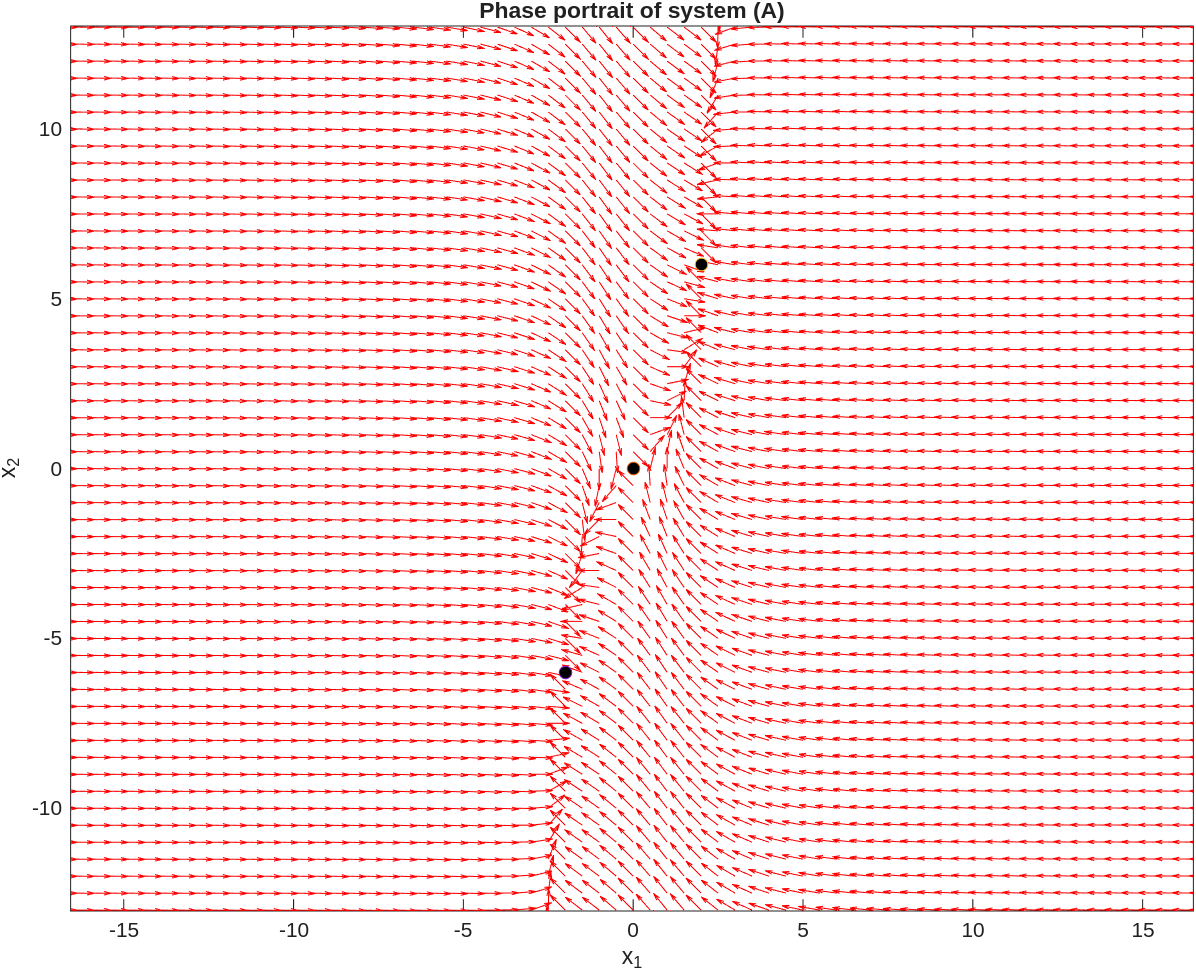
\includegraphics[width=0.7\textwidth]{phase_port_A.png}
    \caption{\textbf{Εικόνα 1.} Φασικό πορτραίτο του συστήματος Α με για τα σημεία ισορροπίας \((x_1, x_2) = (2, 6)\), \((x_1, x_2) = (-2, -6)\) και \((x_1, x_2) = (0, 0)\).}
\end{figure}

\subsubsection{Χρησιμοποιώντας γραμμικοποίηση, μελέτησε την ευστάθεια κάθε σημείου ισορροπίας.}
Ο πίνακας \(\textbf{A}\) για το παραπάνω σύστημα είναι:

\hfill\break
\begin{math}
    \textbf{A} =
    \begin{bmatrix}
        \frac{\partial f_1(x)}{\partial x_1} & \frac{\partial f_1(x)}{\partial x_2} \\
        \frac{\partial f_2(x)}{\partial x_1} & \frac{\partial f_2(x)}{\partial x_2}
    \end{bmatrix} =
    \begin{bmatrix}
        1 - 3x_1^2 &  1 \\
                 3 & -1
    \end{bmatrix}
\end{math}, ο οποίος γύρω από το σημείο ισορροπίας:

\begin{itemize}
    \item \((x_1^1, x_2^1) = (0, 0)\) είναι
    \begin{math}
        \textbf{A} =
        \begin{bmatrix}
            1 &  1 \\
            3 & -1
        \end{bmatrix}
    \end{math}.
    
    \hfill\break
    Το σύστημα \(\dot{\textbf{x}} = \textbf{A}\textbf{x}\) είναι γραμμικό γύρω από αυτό το σημείο ισορροπίας και οι ιδιοτιμές του πίνακα \(\textbf{Α}\) είναι: \((λ-1)(λ+1)-(-1)(-3) = 0 \Rightarrow λ^2 - 1 - 3 = 0 \Rightarrow λ^2 - 4 = 0 \Rightarrow λ_1 = 2, λ_2 = -2\).  Εφόσον μία ιδιοτιμή βρίσκεται στο δεξί μιγαδικό ημιεπίπεδο το σύστημα είναι ασταθές.
    \item \((x_1^2, x_2^2) = (2, 6)\) είναι
    \begin{math}
        \textbf{A} =
        \begin{bmatrix}
            -11 &  1 \\
              3 & -1
        \end{bmatrix}
    \end{math}.
    
    \hfill\break
    Το σύστημα \(\dot{\textbf{x}} = \textbf{A}\textbf{x}\) είναι γραμμικό γύρω από αυτό το σημείο ισορροπίας και οι ιδιοτιμές του πίνακα \(\textbf{Α}\) είναι: \((λ+11)(λ+1)-(-1)(-3) = 0 \Rightarrow λ^2 + λ + 11λ + 11 - 3 = 0 \Rightarrow λ^2 + 12λ + 8 = 0 \Rightarrow λ_1 = -0.7085, λ_2 = -11.2915\). Άρα, ο \(\textbf{A}\) είναι Hurwitz και το σύστημα είναι ασυμπτωτικά ευσταθές.
    item \((x_1^3, x_2^3) = (-2, -6)\) είναι
    \begin{math}
        \textbf{A} =
        \begin{bmatrix}
            -11 &  1 \\
              3 & -1
        \end{bmatrix}
    \end{math}, άρα το σύστημα και γι' αυτό το σημείο ισορροπίας είναι ασυμπτωτικά ευσταθές.
\end{itemize}

\subsubsection{Χρησιμοποιώντας τετραγωνικές συναρτήσεις Lyapunov (quadratic Lyapunov functions), προσέγγισε την περιοχή ελγκτικότητας για κάθε ασυμπτωτικά ευσταθές σημείο ισορροπίας. Προσπάθησε να κάνεις την εκτίμησή σου όσο το δυνατόν μεγαλύτερη.}
Ως περιοχή ελγκτικότητας ορίζουμε \(\Omega_c = \{V(\textbf{x}) < c\}\), όπου \(\textbf{x} = \begin{bmatrix}x_1\\x_2\end{bmatrix}\). Πρακτικά, είναι η περιοχή εκείνη από την οποία αν ξεκινήσει μία τροχιά, δε θα ξεφύγει ποτέ και πάντα θα καταλήγει στο σημείο ισορροπίας. Έτσι, για κάθε ασυμπτωτικά ευσταθές σημείο ισορροπίας θα μελετήσουμε ξεχωριστά την περιοχή ελγκτικότητάς του. Πριν από αυτό όμως, πρέπει να μετασχηματίσουμε το σύστημά μας έτσι ώστε τα ασυμπτωτικά ευσταθή σημεία ισορροπίας να είναι \((y_1, y_2) = (0, 0)\), για να ισχύει η θεωρία ευστάθειας Lyapunov και να μπορούμε να προσδιορίσουμε κατάλληλη συνάρτηση Lyapunov για η μελέτη της περιοχής ελγκτικότηας.  

\hfill\break
Για το σημείο ισορροπίας \((x_1^1, x_2^1) = (2, 6)\) έχουμε:

\hfill\break
\begin{math}
    y_1 = x_1 - 2 \Rightarrow x_1 = y_1 + 2 \\
    y_2 = x_2 - 6 \Rightarrow x_2 = y_2 + 6 \\
    \dot{(y_1 + 2)} = (y_1 + 2) - (y_1 + 2)^3 + (y_2 + 6) \Rightarrow \dot{y}_1 = y_1 + y_2 - (y_1 + 2)^3 + 8 = f_1^{'}(y_1, y_2)\\
    \dot{(y_2 + 6)} = 3(y_1 + 2) - (y_2 + 6) \Rightarrow \dot{y}_2 = 3y_1 - y_2 = f_2^{'}(y_1, y_2)\\
\end{math}

\hfill\break
και επιλέγουμε τη συνάρτηση Lyapunov

\begin{equation*}
    V(y_1, y_2) = y_1^2 + y_2^2
\end{equation*}

\hfill\break
η οποία είναι θετικά ορισμένη, με συνεχείς πρώτες μερικές παραγώγους και η πρώτη παράγωγός της ως προς τον χρόνο είναι:

\begin{equation*}
    \dot{V}(y_1, y_2) = 2y_1\dot{y_1} + 2y_2\dot{y_2} = 2y_1(y_1 + y_2 - (y_1 + 2)^3 + 8) + 2y_2(3y_1 - y_2)
\end{equation*}

\hfill\break
η οποία καταλήγει σε μορφή τέτοια ώστε το πρόσημό της να εξαρτάται από τις τιμές των μεταβλητών \(y_1, y_2\). Με τη βοήθεια της MATLAB ελέγχουμε για δίσκους διαφορετικών ακτινών (\(\sqrt{c}\)) αν όλες οι τιμές εντός τους ικανοποιούν τις συνθήκες: \(V(y_1, y_2) > 0\) και \(\dot{V}(y_1, y_2) \leq 0\). Όσο αυτό ισχύει, αυξάνουμε το \(c\) και ελέγχουμε έναν μεγαλύτερο δίσκο από τον προηγούμενο. Ο έλεγχος σταματά όταν πάψουν να ισχύουν οι συνθήκες. Έτσι, προσδιορίζουμε τη μέγιστη δυνατή περιοχή ελγκτικότητας, για την οποία \(c = 8\).

\hfill\break
Αντίστοιχα, για το σημείο ισορροπίας \((x_1^1, x_2^1) = (-2, -6)\) έχουμε:

\hfill\break
\begin{math}
    y_1 = x_1 + 2 \Rightarrow x_1 = y_1 - 2 \\
    y_2 = x_2 + 6 \Rightarrow x_2 = y_2 - 6 \\
    \dot{(y_1 - 2)} = (y_1 - 2) - (y_1 - 2)^3 + (y_2 - 6) \Rightarrow \dot{y}_1 = y_1 + y_2 - (y_1 - 2)^3 - 8 = f_1^{'}(y_1, y_2)\\
    \dot{(y_2 - 6)} = 3(y_1 - 2) - (y_2 - 6) \Rightarrow \dot{y}_2 = 3y_1 - y_2 = f_2^{'}(y_1, y_2)\\
\end{math}

\hfill\break
και επιλέγουμε τημ ίδια συνάρτηση Lyapunov με πριν, η οποία είναι θετικά ορισμένη, με συνεχείς πρώτες μερικές παραγώγους και η πρώτη παράγωγός της ως προς τον χρόνο είναι:

\begin{equation*}
    \dot{V}(y_1,y_2) = 2y_1\dot{y}_1 + 2y_2\dot{y_2}
\end{equation*}

\hfill\break
Με τον ίδιο τρόπο προκύπτει η περιοχή ελγκτικότητας να είναι ένας δίσκος με ακτίνα 8.

\begin{figure}[h]
    \centering
    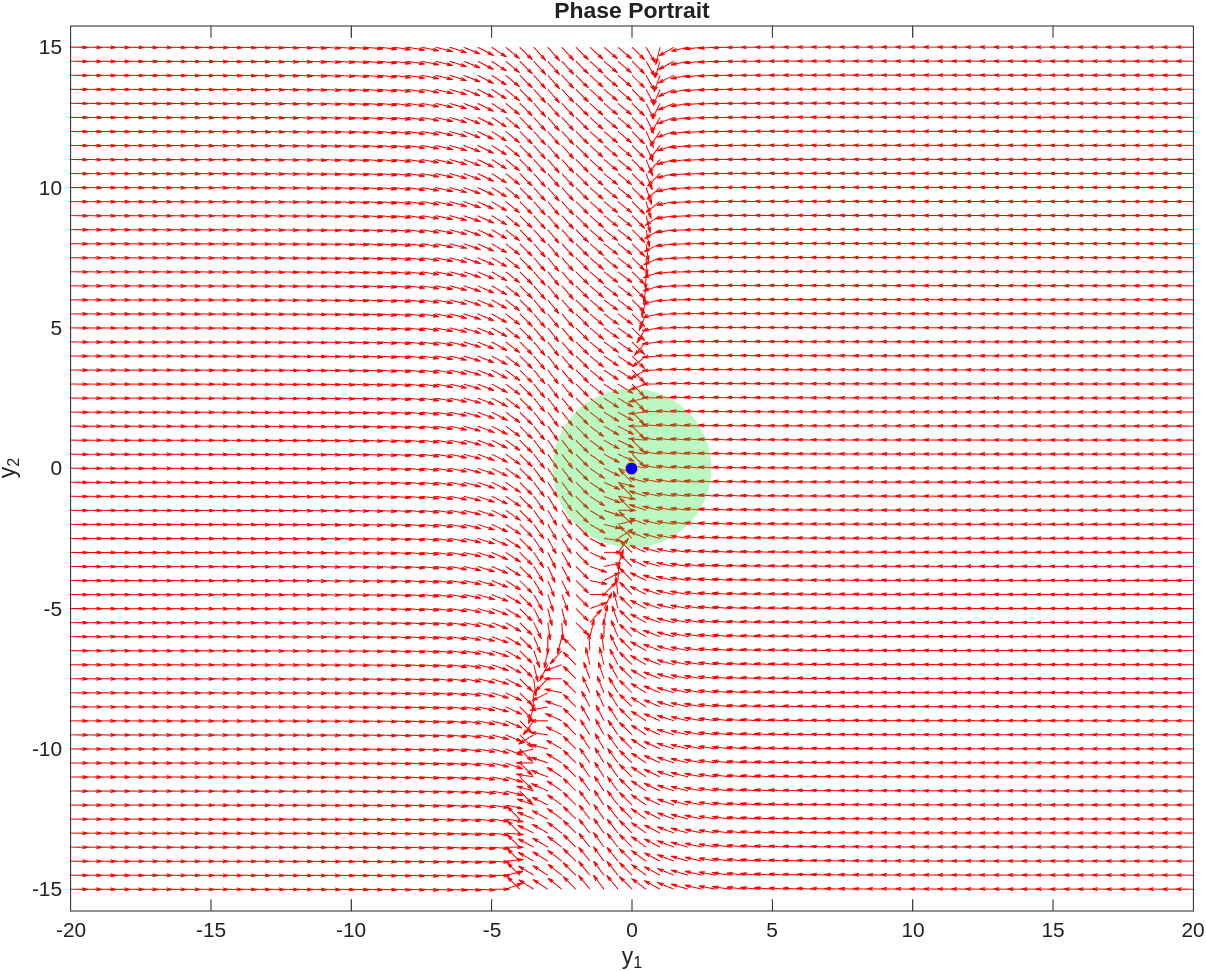
\includegraphics[width=0.7\textwidth]{phase_port_A1A2_ROA_real.png}
    \caption{\textbf{Εικόνα 2.} Φασικό πορτραίτο του συστήματος Α, για τα σημεία ισορροπίας \((x_1, x_2) = (2, 6)\) και \((x_1,x_2) = (-2, -6)\), που στο μετασχηματισμένο σύστημα αντιστοιχούν στο σημείο \((y_1, y_2) = (0, 0)\), με την βέλτιστη περιοχή ελγκτικότητας να είναι ο πράσινος δίσκος, ακτίνας \(\sqrt{c} = 2.828\).}
\end{figure}

\subsubsection{Κατασκευάστε το φασικό πορτραίτο του συστήματος και δείξτε σε αυτό τις ακριβείς περιοχές ελγκτικότητας καθώς και την εκτίμησή σας, όπως βρέθηκε πριν.}
Κοιτώντας το φασικό πορτραίτο του συστήματος θα μπορούσαμε να πούμε ότι η περιοχή ελγκτικότητας είναι ένας κύκλος μεγαλύτερης ακτίνας από αυτό που προσδιορίσαμε πριν. Δοκιμάζοντας τον δίσκο με σταθερά \(c = 8.01\), που η διαφορά από πριν είναι ελάχιστη, μπορούμε να παρατηρήσουμε τα εξής:

\begin{figure}[h!]
    \centering
    \begin{subfigure}{0.45\textwidth}
        \centering
        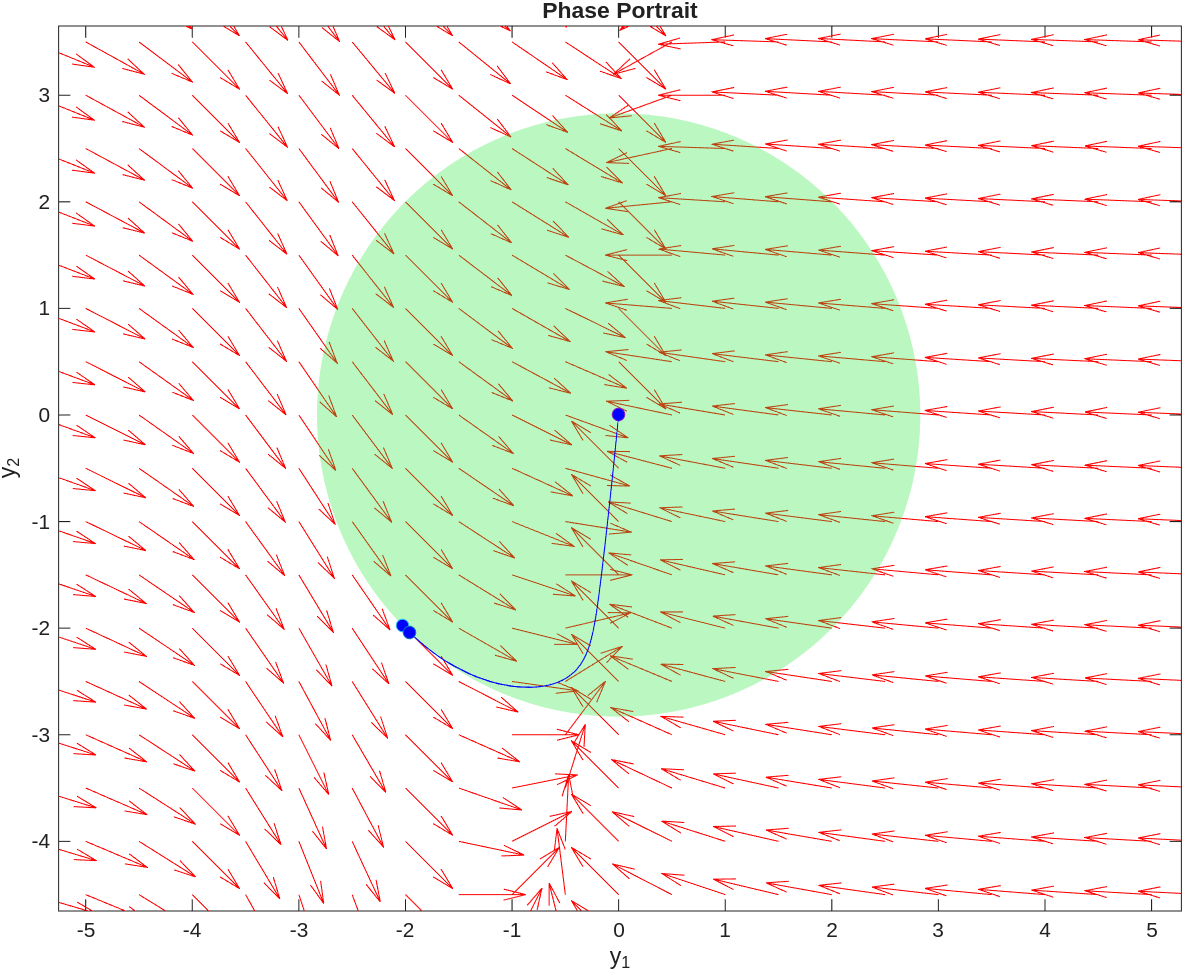
\includegraphics[width=\textwidth]{phase_port_A1_ROA_801a.png}
        \caption{\textbf{Εικόνα 3.1.} Στην εικόνα βλέπουμε την περιοχή ελγκτικότητας για σταθερά \(c = 8.01\). Τα δύο σημεία στην περιφέρεια του δίσκου, που απεικονίζονται με μπλε, είναι αυτά για το οποία δεν ισχύει \(\dot{V}(y_1, y_2) \leq 0\).}
    \end{subfigure}
    \,\,\,\,\,\,
    \begin{subfigure}{0.45\textwidth}
        \centering
        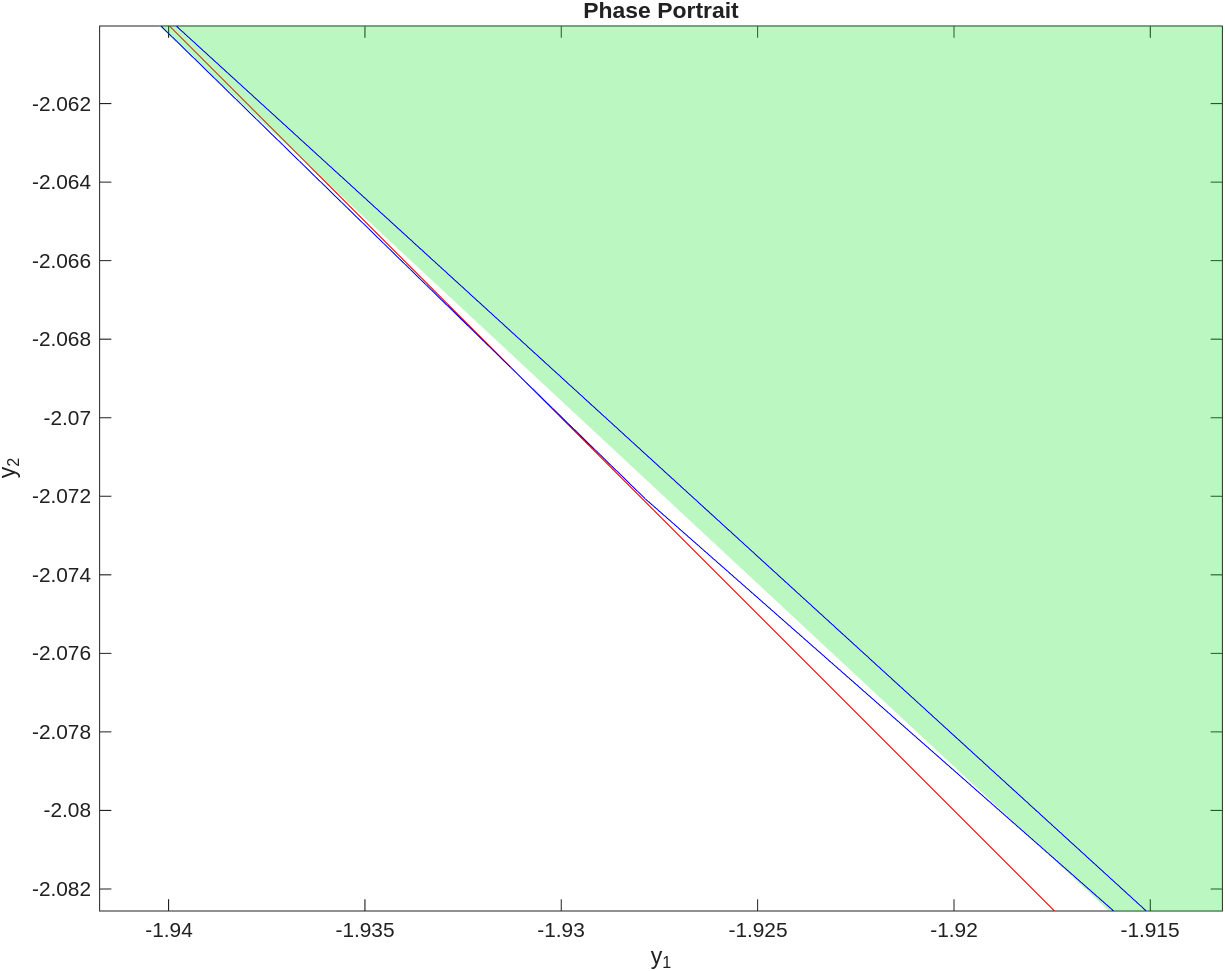
\includegraphics[width=\textwidth]{phase_port_A1_ROA_801b.png}
        \caption{\textbf{Εικόνα 3.2.} Για τα σημεία της περιφέρειας του κύκλου της Εικόνας 2.1 μπορούμε να διαπιστώσουμε πως, ενώ οι τροχιές καταλήγουν στο σημείο ισορροπίας, βγαίνουν εκτός του δίσκου που ορίζεται από την περιοχή ελγκτικότητας.}
    \end{subfigure}
\end{figure}

\hfill\break
Αν δοκιμάσουμε \(c = 12\), δηλαδή ακόμη μεγαλύτερο, θα δούμε ότι οι τροχιές ορισμένων σημείων ξεφεύγουν εντελώς από τον δίσκο και αυτό είναι εμφανές χωρίς να εστιάσουμε κοντά στην εκάστοτε τροχιά.

\begin{figure}[h!]
    \centering
    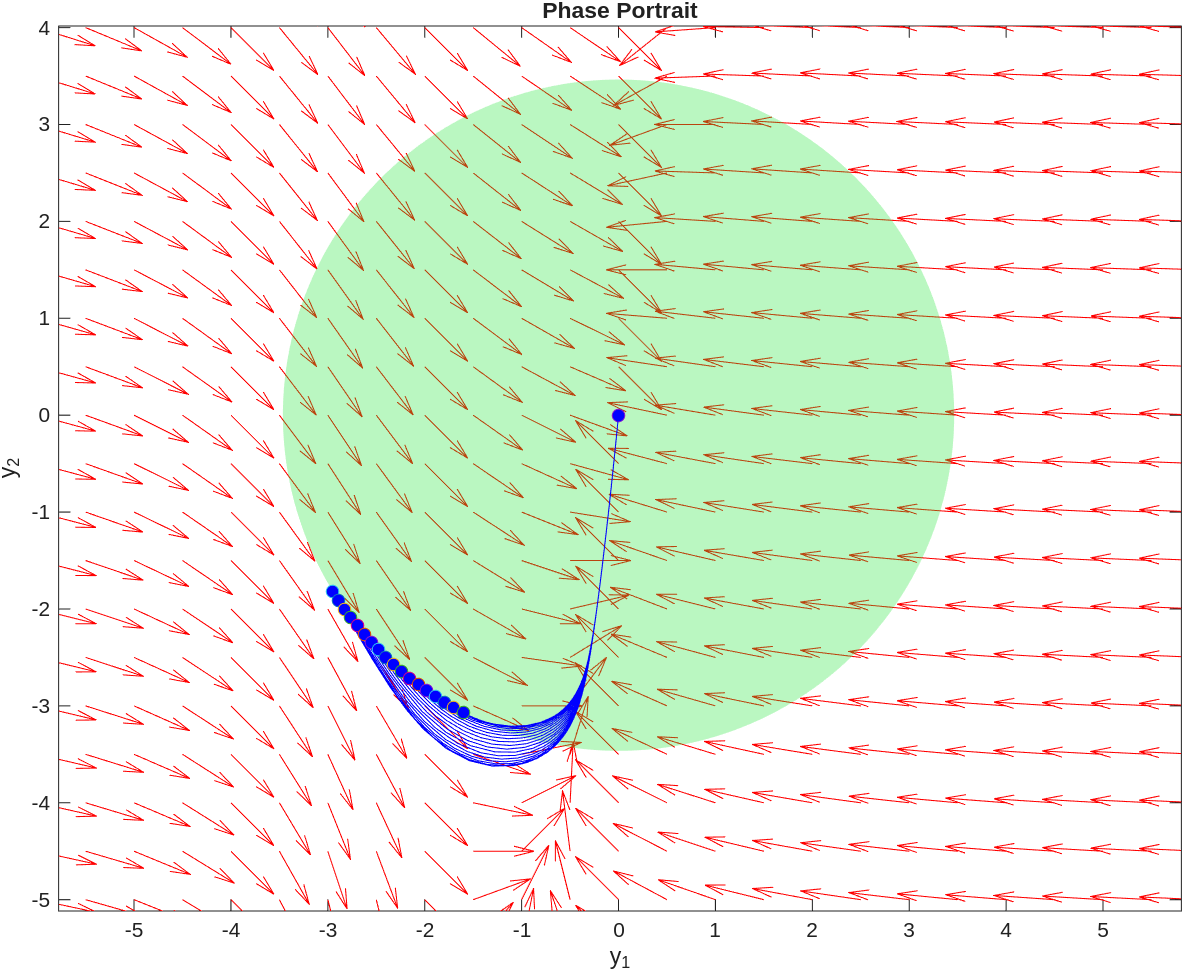
\includegraphics[width=0.7\textwidth]{phase_port_A1_ROA_12.png}
    \caption{\textbf{Εικόνα 4.} Στην εικόνα βλέπουμε την περιοχή ελγκτικότητας για σταθερά \(c = 12\). Τα σημεία που απεικονίζονται στην περιφέρεια του δίσκου, είναι αυτά για το οποία δεν ισχύει \(\dot{V}(y_1, y_2) \leq 0\).}
\end{figure}

\hfill\break
Αν μεγαλώσουμε κι άλλο την τιμή \(c\), οι τροχιές ξεφεύγουν ακόμα περισσότερο. Άρα, η βέκτιστη τιμή είναι το \(8\). Αυτό γίνεται ακόμη πιο ξεκάθαρο με τη βοήθεια της παρακάτω εικόνας.

\hfill\break
\begin{figure}[h!]
    \centering
    
\includegraphics[width=0.9\textwidth]{GeoGebra_sysA.png}
    \caption{\textbf{Εικόνα 5.} (μπεζ) Η συνάρτηση Lyapunov. (ροζ) Η χρονική παράγωγος της συνάρτησης Lyapunov. (μπλε) Ο δίσκος ακτίνας \(\sqrt{c} = \sqrt{8}\). Αν η σταθερά \(c\) αυξηθεί ο δίσκος θα περιλαμβάνει σημεία στα οποία η χρονική παράγωγος της V παίρνει θετικές τιμές.}
\end{figure}

\subsection{Σύστημα (Β)}
Δίνεται το σύστημα:

\begin{equation*}
    \dot{x}_1 = -\frac{1}{2}\tan(\frac{\pi x_1}{2}) + x_2 = f_1(x_1, x_2)
\end{equation*}

\begin{equation*}
    \dot{x}_2 = x_1 - \frac{1}{2}\tan(\frac{\pi x_2}{2}) = f_2(x_1, x_2)
\end{equation*}

\subsubsection{Να βρεθούν τα σημεία ισορροπίας (equilibrium points) του συστήματος.}
Τα σημεία ισορροπίας του συγκεκριμένου συστήματος είναι άπειρα σε όλο τον χώρο, επομένως πάμε να μελετήσουμε τι συμβαίνει γύρω από το \((x_1, x_2) = (0, 0)\). Για τον σκοπό αυτό θα αξιοποιήσουμε το φασικό πορτραίτο του συστήματος.

\begin{figure}[h]
    \centering
    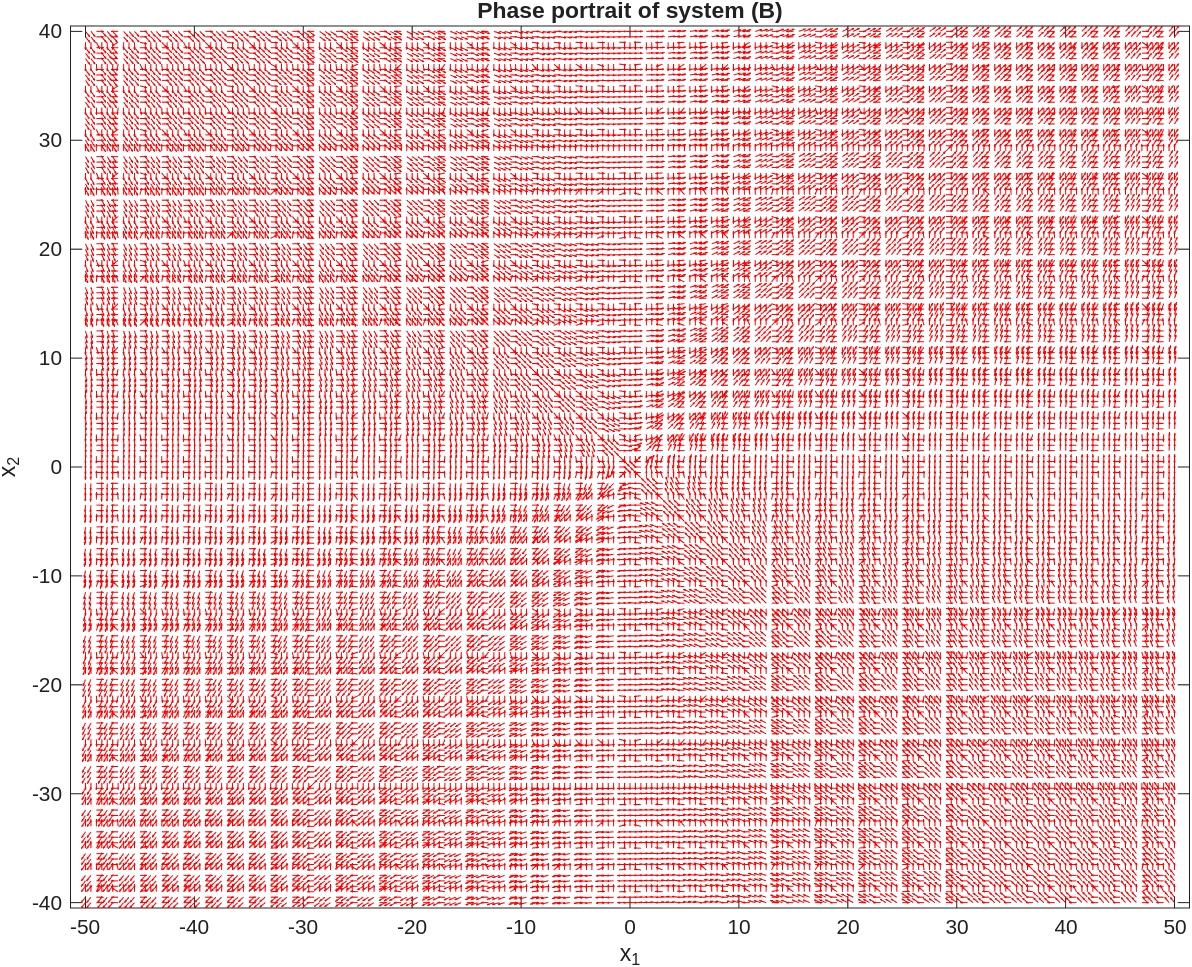
\includegraphics[width=0.7\textwidth]{phase_port_B.png}
    \caption{\textbf{Εικόνα 6.} Φασικό πορτραίτο του συστήματος B.}
\end{figure}

\hfill\break
Θέτοντας ως αρχικές συνθήκες για το σύστημα -διαδοχικά- τα σημεία:

\hfill\break
\begin{math}
    (x_1, x_2) = (0.2, -0.3) \\[10pt]
    (x_1, x_2) = (-0.1, 0.4) \\[10pt]
    (x_1, x_2) = (0.03, 0.03)
\end{math}

\hfill\break
και έχοντας βρει τα σημεία ισορροπίας για το σύστημα κοντά σε αυτές τις αρχικές συνθήκες ως:

\hfill\break
\begin{math}
    (x_1^1, x_2^1) = (0, 0) \\[10pt]
    (x_1^2, x_2^2) = (-0.5, 0.5) \\[10pt] 
    (x_1^3, x_2^3) = (0.5, -0.5)
\end{math}

\hfill\break
παρατηρούμε ότι οι τροχίες καταλήγουν πάντα στα δύο πρώτα σημεία ισορροπίας, ποτέ στο μηδενικό, όσο κοντά και αν διαλέξουμε την αρχική συνθήκη. Έτσι, μπορούμε να συμπεράνουμε πως το μηδενικό σημείο ισορροπίας είναι ασταθές.

\begin{figure}[h]
    \centering
    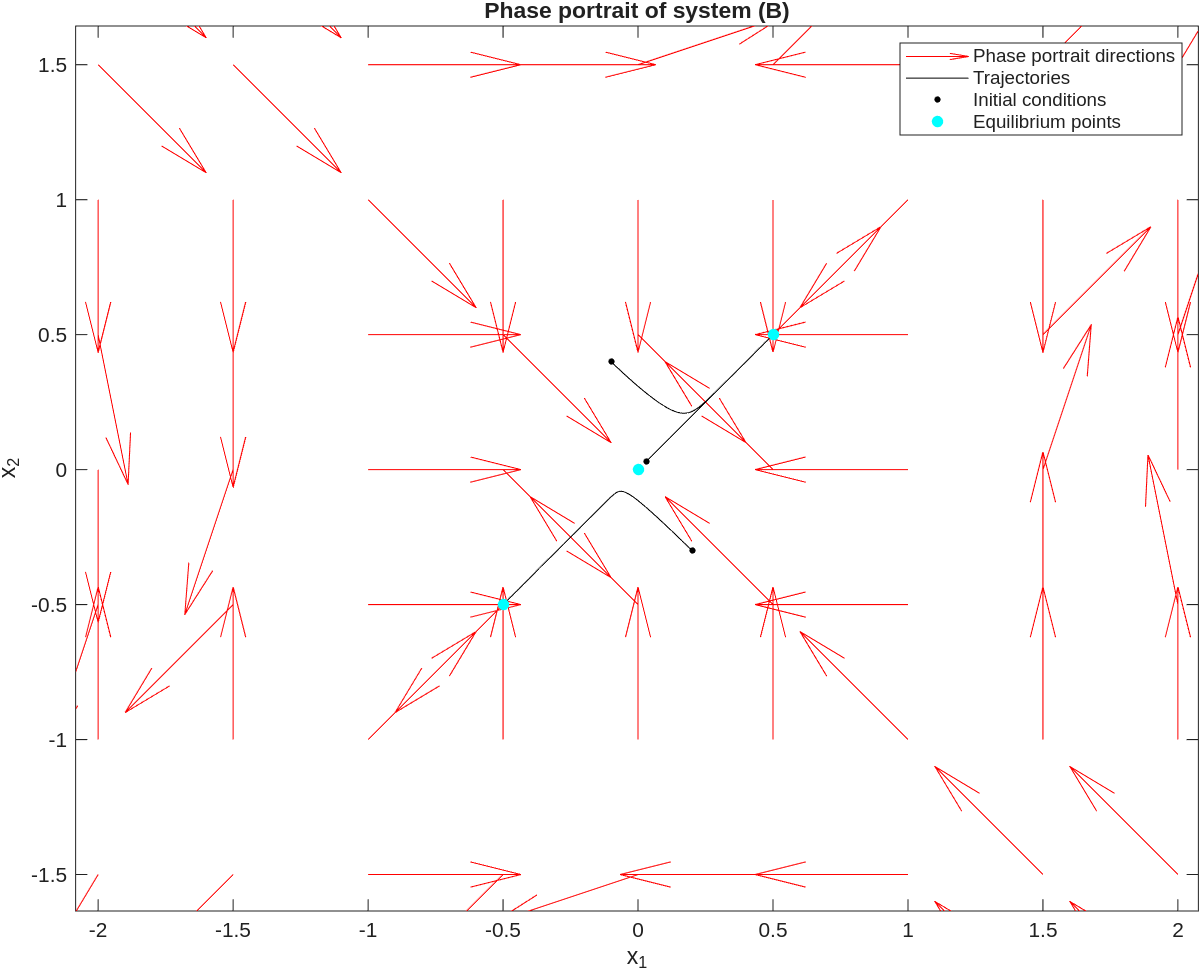
\includegraphics[width=0.7\textwidth]{phase_port_B_ep.png}
    \caption{\textbf{Εικόνα 7.} Σημεία ισορροπίας και αρχικές συνθήκες, όπως ορίστηκαν παραπάνω και οι τροχιές που ακολουθεί το σύστημα ξεκινώντας από τις δεδομένες αρχικές συνθήκες.}
\end{figure}

\subsubsection{Χρησιμοποιώντας γραμμικοποίηση, μελέτησε την ευστάθεια κάθε σημείου ισορροπίας.}
Ο πίνακας \(\textbf{A}\) για το παραπάνω σύστημα είναι:

\hfill\break
\begin{math}
    \textbf{A} =
    \begin{bmatrix}
        \frac{\partial f_1(x)}{\partial x_1} & \frac{\partial f_1(x)}{\partial x_2} \\
        \frac{\partial f_2(x)}{\partial x_1} & \frac{\partial f_2(x)}{\partial x_2}
    \end{bmatrix} =
    \begin{bmatrix}
        -\frac{\pi}{4} sec^2(\frac{\pi x_1}{2}) &                                      1 \\
                                              1 & -\frac{\pi}{4} sec^2(\frac{\pi x_2}{2})
    \end{bmatrix}
\end{math}, ο οποίος γύρω από το σημείο ισορροπίας:

\begin{itemize}
    \item \((x_1^1, x_2^1) = (0, 0)\) είναι
    \begin{math}
        \textbf{A} =
        \begin{bmatrix}
            -\pi/4 &      1 \\
                 1 & -\pi/4
        \end{bmatrix}
    \end{math}.
    
    \hfill\break
    Το σύστημα \(\dot{\textbf{x}} = \textbf{A}\textbf{x}\) είναι γραμμικό γύρω από αυτό και οι ιδιοτιμές είναι:\\[10pt]
    \begin{math}
        (λ + \pi /4) (λ + \pi /4) - (-1) (-1) = 0 \Rightarrow \\[10pt]
        λ^2 + 2λ\frac{\pi}{4} + (\frac{\pi}{4})^2 - 1 = 0 \Rightarrow \\[10pt]
        λ^2 + λ\frac{\pi}{2} + \frac{\pi^2}{16} - \frac{16}{16} = 0 \Rightarrow \\[10pt]
        λ^2 + λ\frac{\pi}{2} + \frac{\pi^2 - 16}{16} = 0 \Rightarrow \\[10pt]
        16 λ^2 + (8 \pi) λ + (\pi^2 - 16) = 0 \Rightarrow \\[10pt]
        λ_1 = -6.1304\,\,\,\texttt{ή}\,\,\, λ_2 = 0.2146 \\[10pt]
    \end{math}
    Εφόσον μία ιδιοτιμή βρίσκεται στο δεξί μιγαδικό ημιεπίπεδο το σύστημα είναι ασταθές γύρω από αυτό το σημείο ισορροπίας.
    \item \((x_1^2, x_2^2) = (-0.5, 0.5)\) είναι
    \begin{math}
        \textbf{A} =
        \begin{bmatrix}
            -\pi/2 &      1 \\
                 1 & -\pi/2
        \end{bmatrix}
    \end{math}.
    
    \hfill\break
    Το σύστημα \(\dot{\textbf{x}} = \textbf{A}\textbf{x}\) είναι γραμμικό γύρω από αυτό και οι ιδιοτιμές είναι:\\[10pt]
    \begin{math}
        (λ + \pi/2) (λ + \pi /2) - (-1) (-1) = 0 \Rightarrow \\[10pt]
        (λ + \pi/2)^2 - 1 = 0 \Rightarrow \\[10pt]
        (λ + \pi/2)^2 = 1 \Rightarrow \\[10pt]
        λ + \pi/2 = \pm 1 \Rightarrow \\[10pt]
        λ_1 = 1 - \pi/2 < 0\,\,\,\texttt{ή}\,\,\, λ_1 = - 1 - \pi/2 < 0\\[10pt]
    \end{math}
    Αφού και οι δύο ιδιοτιμές είναι αρνητικές, το σημείο ισορροπίας είναι ασυμπτωτικά ευσταθές.
    \item \((x_1^2, x_2^2) = (0.5, -0.5)\) είναι
    \begin{math}
        \textbf{A} =
        \begin{bmatrix}
            -\pi/2 &      1 \\
                 1 & -\pi/2
        \end{bmatrix}
    \end{math}.
    
    \hfill\break
    Με όμοιο τρόπο προκύπτουν οι ίδιες ιδιοτιμές και το σημείο ισορροπίας είναι και αυτό ασυμπτωτικά ευσταθές.
\end{itemize}

\subsubsection{Χρησιμοποιώντας τετραγωνικές συναρτήσεις Lyapunov (quadratic Lyapunov functions), προσέγγισε την περιοχή ελγκτικότητας για κάθε ασυμπτωτικά ευσταθές σημείο ισορροπίας. Προσπάθησε να κάνεις την εκτίμησή σου όσο το δυνατόν μεγαλύτερη.}
Πρέπει και εδώ, όπως και στο σύστημα Α, να κάνουμε έναν μετασχηματισμό, έτσι ώστε τα ασυμπτωτικά ευσταθή σημεία ισορροπίας να είναι \((y_1, y_2) = (0, 0)\).

\hfill\break
Για το σημείο ισορροπίας \((x_1^2, x_2^2) = (-0.5, 0.5)\) έχουμε:

\hfill\break
\begin{math}
    y_1 = x_1 + 0.5 \Rightarrow x_1 = y_1 - 0.5 \\
    y_2 = x_2 - 0.5 \Rightarrow x_2 = y_2 + 0.5 \\
    \dot{(y_1 - 0.5)} = (y_2 + 0.5) - \frac{1}{2}\tan(\frac{\pi (y_1 - 0.5)}{2}) 
    \Rightarrow \dot{y}_1 = y_2 - \frac{1}{2}\tan(\frac{\pi (y_1 - 0.5)}{2}) + 0.5 = f_1^{'}(y_1, y_2)\\
    \dot{(y_2 + 0.5)} = (y_1 - 0.5) - \frac{1}{2}\tan(\frac{\pi (y_2 + 0.5)}{2})
    \Rightarrow \dot{y}_2 = y_1 - \frac{1}{2}\tan(\frac{\pi (y_2 + 0.5)}{2}) - 0.5 = f_2^{'}(y_1, y_2)
\end{math}

\hfill\break
και επιλέγουμε τη συνάρτηση Lyapunov

\begin{equation*}
    V(y_1, y_2) = y_1^2 + y_2^2
\end{equation*}

\hfill\break
η οποία είναι θετικά ορισμένη, με συνεχείς πρώτες μερικές παραγώγους και η πρώτη παράγωγός της ως προς τον χρόνο είναι:

\begin{equation*}
    \dot{V}(y_1, y_2) = 2y_1\dot{y_1} + 2y_2\dot{y_2}
\end{equation*}

\hfill\break
η οποία καταλήγει σε μορφή τέτοια ώστε το πρόσημό της να εξαρτάται από τις τιμές των μεταβλητών \(y_1, y_2\). Με τη βοήθεια της MATLAB ελέγχουμε για δίσκους διαφορετικών ακτινών (\(\sqrt{c}\)) και βρίσκουμε τη μέγιστη δυνατή περιοχή ελγκτικότητας, για την οποία τελικά φαίνεται να μην υπάρχει περιοχή ελγκτικότητας. Το ίδιο ισχύει και για το σημείο ισορροπίας \((x_1^3, x_2^3) = (0.5, -0.5)\)

\section{Άσκηση 4η}
Δίνεται το σύστημα
\begin{equation*}
    \dot x = -a(I_n + S(x) + x x^T)x,\qquad a>0,
\end{equation*}

\hfill\break
Επιλέγουμε ως συνάρτηση Lyapunov την
\begin{equation*}
    V(x)=\frac{1}{2}x^Tx
\end{equation*}

\hfill\break
η οποία είναι θετικά ορισμένη, με συνεχή πρώτη μερική παράγωγο και η παράγωγος ως προς το χρόνο είναι:

\begin{align*}
    \dot V(x)
    &= \frac{d}{dt}\!\left(\tfrac{1}{2}x^{T}x\right)
    = \tfrac{1}{2}\big(\dot x^{T}x + x^{T}\dot x\big)
    = x^{T}\dot x \\
    &= x^{T}\Big[-a\big(I_n + S(x) + x x^{T}\big)x\Big] \\
    &= -a\,x^{T}\big(I_n + S(x) + x x^{T}\big)x \\
    &= -a\big(x^{T}I_n x + x^{T}S(x)x + x^{T}(x x^{T})x\big).
\end{align*}

\hfill\break
Εξετάζοντας κάθε όρο ξεχωριστά έχουμε: 

\begin{itemize}
  \item \(-α(x^T I_n x) = -α x^T x\),
  \item η \(S(x)\) είναι skwe-symmetric, άρα θα ισχύει \(S(x)^T = -S (x)\), επομένως: \newline
  \(-a(x^T S(χ) x) = a(x^T (-S(x)) x) = a(x^T S(x)^T x) = a(x^T S(x) x)^T\). Όμως, ο όρος \(-a(x^T S(s) x)\) είναι βαθμωτός (\((n \times 1)^T \times (n \times n) \times (n \times 1) = (1 \times n) \times (n \times n) \times (n \times 1) = (1 \times 1)\), και εφόσον είναι ίσος και αντίθετος με τον εαυτό του, αναγκαστικά πρέπει να είναι 0,
  \item \(x^T(x x^T)x = (x^T x)(x^T x) = (x^T x)^{2}\).
\end{itemize}

\hfill\break
Έτσι, καταλήγουμε:

\hfill\break
\begin{math}
    \dot{V}(x) = -a (x^T x) + 0 - a(x^T x)^2 = -a ((x^T x) + (x^T x)^2) = -2a (\frac{x^T x}{2} + \frac{(x^T x)^2}{2}) = -2a (V(x) + K(x))
\end{math}, όπου \(K(x) \geq 0,\,\,\forall x = x(t)\), άρα

\begin{math}
    \dot{V}(x(t)) \leq -2a V(x(t)) \Rightarrow V(x(t)) \leq e^{-2at} V(x(0))
\end{math}

\hfill\break
Γνωρίζουμε ότι ο όρος \(x^T x\) είναι η τετραγωνική νόρμα του διανύσματος x=x(t) (\(\|x\|^2\)). Έτσι, ισχύει:

\hfill\break
\begin{math}
    2\frac{1}{2}\|x\|^{2} = 2\frac{1}{2}x^T x = 2V(x(t)) \le 2e^{-2a t}V(x(0)) = e^{-2a t}\|x(0)\|^{2}
\end{math},

\hfill\break
δηλαδή

\hfill\break
\begin{math}
    \|x(t)\|^2 \le e^{-2at}\|x(0)\|^2 \Rightarrow
    \sqrt{\|x(t)\|^2} \leq \sqrt{e^{-2at}\|x(0)\|^2} \Rightarrow
    \|x(t)\| \le e^{-at}\|x(0)\|\,\,\, (1)
\end{math}

\hfill\break
Τελικά, το σύστημά μας είναι ολικά, εκθετικά ευσταθές, καθώς η ανίσωση (1) ισχύει για κάθε αρχική κατάσταση \(x(0)\), χωρίς κανέναν περιορισμό, \(\forall t \geq 0\) και ο ρυθμός εκθετικής μείωσης της παράστασης είναι ίσος με τη σταθερά \(a\).

\section{Άσκηση 5η}
Δίνεται το σύστημα
\begin{equation*}
    \dot{x} = f(x) + G(x)u,\,\,\,x \in \mathbb{R}^n    
\end{equation*}

\hfill\break
και δίνεται ότι υπάρχει συμμετρικός, θετικά ορισμένος πίνακας \(P = P^T > 0\), μια συνάρτηση \(W(x)\ge 0\) και θετικές σταθερές \(\gamma > 0,\,\,\,\sigma > 0\) που ικανοποιούν \(\forall x \in \mathbb{R}^n\) την ανισότητα
\begin{equation}
    2 x^T P f(x) + \gamma x^T P x + W(x) - 2 \sigma x^T P G(x) G(x)^T P x \le 0.
\end{equation}

\hfill\break
Θέλουμε να σχεδιάσουμε έναν νόμο ελέγχου \(u(x)\), τέτοιο ώστε το Σύστημα Κλειστού Βρόχου (ΣΚΒ) να έχει ολικά, εκθετικά ευσταθές σημείο ισορροπίας. Στην εκφώνηση μας δίνεται ο νόμος ελέγχου, άρα θα πρέπει να αποδείξουμε το ζητούμενο για το \(u = -\sigma G(x)^T P x\). Έτσι, η δυναμική του συστήματος γίνεται:

\begin{align*}
    \dot{x} 
    &= f(x) + G(x) (- \sigma G(x)^T P x) \\
    &= f(x) - \sigma G(x) G(x)^T P x  
\end{align*}

\hfill\break
Επιλέγουμε ως συνάρτηση Lyapunov την:
\begin{equation*}
    V(x) = x^T P x,
\end{equation*}

\hfill\break
η οποία είναι θετικά ορισμένη, αφού από τα δεδομένα έχουμε ότι \(P > 0\). Έπειτα, υπολογίζουμε τη χρονική παράγωγο της \(V\):

\begin{align*}
    \dot{V}(x)
    &= \frac{d}{dt}\big(x^{T}P x\big) \\
    &= 2x^{T}P\dot x \\
    &= 2x^{T}P f(x) + 2x^{T}P G(x)\big(-\sigma G(x)^{T}P x\big) \\
    &= 2x^{T}P f(x) - 2\sigma\, x^{T}P G(x)G(x)^{T}P x.
\end{align*}

\hfill\break
Επιστρέφοντας στην ανίσωση (1):

\hfill\break
\begin{align*}
    (1) \Rightarrow
    &2 x^T P f(x) - 2 \sigma x^T P G(x) G(x)^T P x \leq -\gamma x^T P x - W(x) \\
    \Rightarrow
    &\dot{V}(x) \leq -\gamma x^T P x - W(x) \leq -\gamma x^T P x = - \gamma V(x)
\end{align*}

\hfill\break
αφού από τα δεδομένα ξέρουμε ότι \(W(x) \leq 0\). Άρα, καταλήγουμε στην ανίσωση \(\dot{V}(x) \leq - \gamma V(x)\), η οποία αν ολοκληρώσουμε γίνεται για  \(x = x(t)\): \(V(x(t)) \leq e^{- \gamma t} V(x(0)),\,\,\, t \geq 0\).

\hfill\break
Αξιοποιώντας τις ιδιότητες του πίνακα \(P\), που εγγυώνται ύπαρξη ιδιοτιμών, μπορούμε να γράψουμε:

\hfill\break
\begin{math}
    \lambda_{\min}(P)\|x(t)\|^2 \le V(x(t)) \le \lambda_{\max}(P)\|x(t)\|^2 \Rightarrow \\[10pt]
    \lambda_{\min}(P)\,\|x(t)\|^2 \le V(x(t)) \le e^{-\gamma t}V(x(0)) \le e^{-\gamma t}\lambda_{\max}(P)\|x(0)\|^2 \Rightarrow \\[10pt]
    \|x(t)\|^2 \le \frac{\lambda_{\max}(P)}{\lambda_{\min}(P)}\,e^{-\gamma t}\,\|x(0)\|^2 \Rightarrow \\[10pt]
    \|x(t)\| \le \sqrt{\frac{\lambda_{\max}(P)}{\lambda_{\min}(P)}} e^{-\gamma t/2} \|x(0)\|
\end{math}

\hfill\break
όπου \(\lambda_{\min}\) η ελάχιστη και \(\lambda_{\max}\) η μέγιστη ιδιοτιμή του πίνακα \(P\) και ισχύει \(0 < \lambda_{\min}(P) \le \lambda_{\max}(P)\).

\hfill\break
Τελικά, διαπιστώνουμε ότι το ΣΚΒ είναι ολικά εκθετικά ευσταθές με σταθερό "πλάτος" \(A=\sqrt{\frac{\lambda_{\max}(P)}{\lambda_{\min}(P)}}\) και ρυθμό απόσβεσης \(1/\tau = \frac{\gamma}{2}\), δηλαδή
\[
\|x(t)\| \le Α e^{-\frac{1}{\tau} t}\|x(0)\|.
\]
\end{document}